
\chapter{  Sprint 2 : Gestion des Tâches }

\section*{Introduction}
\addcontentsline{toc}{section}{Introduction}

Dans ce sprint, nous nous concentrons sur le développement des fonctionnalités de création et de consultation des tâches dans notre application. Nous avons élaboré un backlog, des cas d'utilisation, des diagrammes de séquence et des descriptions textuelles pour guider notre travail. Nous avons également conçu un diagramme de classe participantes pour planifier l'implémentation des fonctionnalités, ainsi que des captures d'écran des interfaces utilisateur. Nous examinerons également le burndown chart et le task board pour suivre l'avancement du sprint et discuterons de la mise en œuvre des tests unitaires pour garantir la qualité du code.
%________________________________________________________________________________________________________________

\section{Backlog du sprint 2}


\begin{table}[H]
  \centering
  \renewcommand{\arraystretch}{1} % Facteur d'étirement des lignes
  \begin{tabular}{|c|c|p{7.8cm}|c|}
    \hline
    \textbf{ID}   & \textbf{Fonctionnalités} & \centering \textbf{User Story}                                                                                                                      & \textbf {Story points} \\
    \hline
    \textbf{US6}  & Gestion des véhicules    & En tant qu'administrateur, je veux ajouter, supprimer et visualiser les véhicules pour que la gestion du parc soit efficace et à jour.              & 5                      \\
    \hline
    \textbf{US7}  & Créations des taches     & En tant que Chef d'équipe je veux Créer des taches pour les chauffeurs et les mécanicien.                                                           & 5                      \\
    \hline
    \textbf{US8}  & Consultation des taches  & En tant que Chauffeur je veux consulter la checklist pour que je puisse vérifier tous les éléments essentiels et confirmer l'exécution des tâches . & 3                      \\
    \hline
    \textbf{US9}  & Consultation des taches  & En tant que Mécanicien je veux Consulter les détails des interventions pour que je puisse obtenir toutes les informations sur les tâches assignées. & 3                      \\
    \hline
    \textbf{US10} & Validation des taches    & En tant que Chef d'équipe je veux valider les taches du mécanicien                                                                                  & 3                      \\
    \hline
  \end{tabular}
  \caption{Backlog du sprint 2}

\end{table}

%________________________________________________________________________________________________________________
\newpage
\section{Analyse et conception}

Dans cette section, nous détaillerons le processus d'analyse et de conception pour les fonctionnalités de création et de consultation des tâches.

%________________________________________________________________________________________________________________
\subsection{Diagramme de cas d’utilisation du sprint 2 }

\begin{figure}[h!]
  \centering
  \includegraphics[width=1\textwidth,height=10cm]{chap4.images/dcu global sprint 2.png}
  \caption{Diagramme de cas d’utilisation global du sprint 2}

\end{figure}

%________________________________________________________________________________________________________________
%________________________________________________________________________________________________________

\subsection{Raffinement du cas d'utilisation « Gérer les véhicules »}

\begin{figure}[h!]
  \centering
  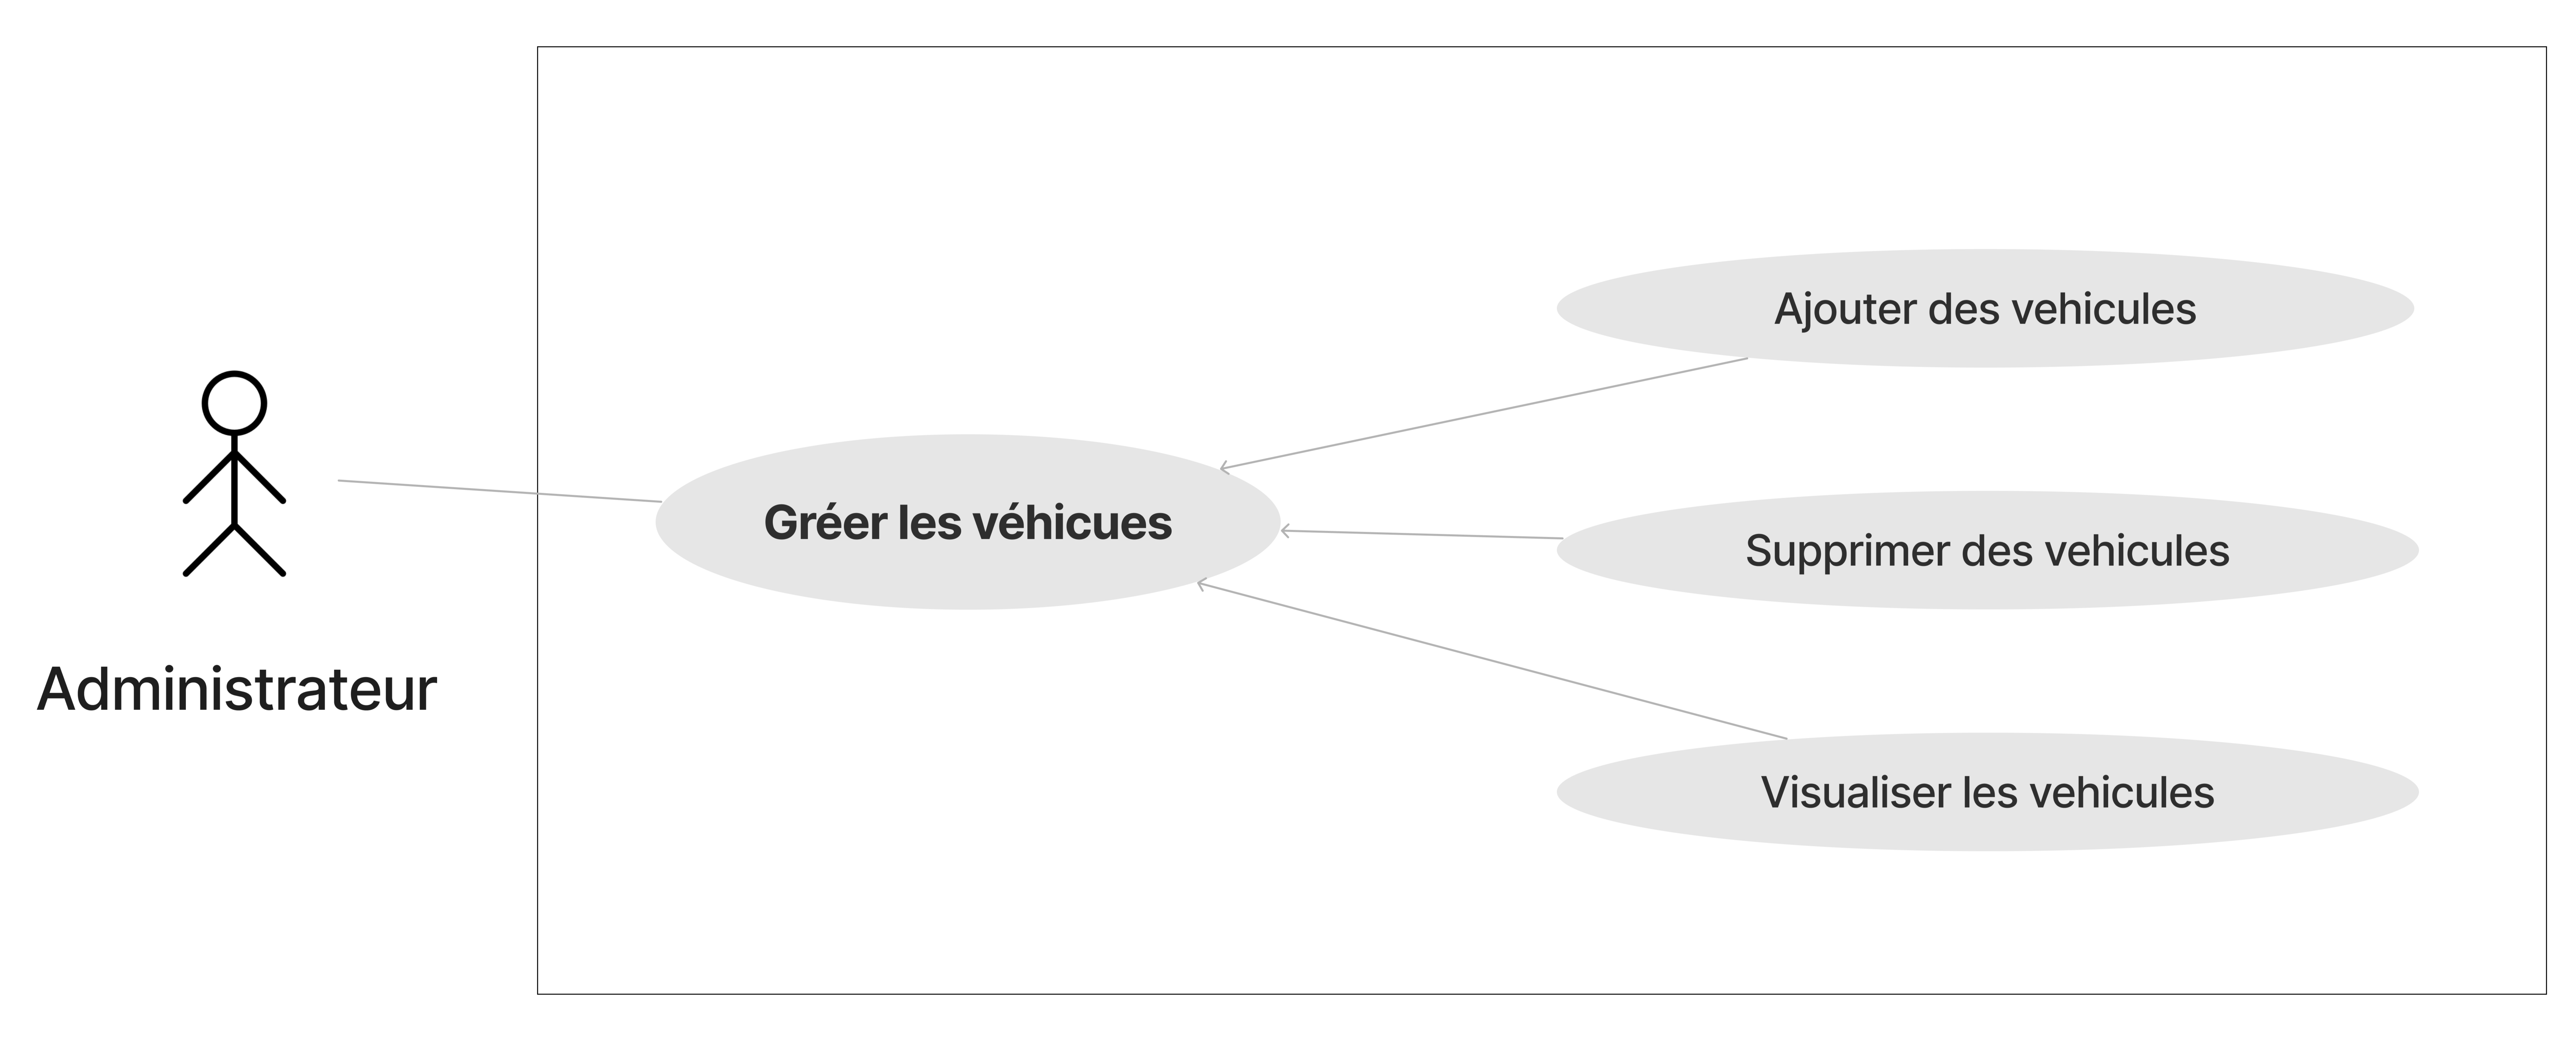
\includegraphics[width=1\textwidth,height=6cm]{chap4.images/raf Gérer les véhicules.png}
  \caption{Raffinement de cas d’utilisation « Gérer les véhicues »}

\end{figure}


%________________________________________________________________________________________________________________

\subsection{Description textuelle du cas d’utilisation « Ajouter véhicules »}

\begin{table}[H]
  \centering
  \renewcommand{\arraystretch}{1.2} % Facteur d'étirement des lignes
  \begin{tabular}{|p{4cm}|p{9cm}|}
    \hline
    \textbf{Cas d'utilisation}   & Ajouter des Véhicules                                                                    \\
    \hline
    \textbf{Acteur}              & Administrateur                                                                           \\
    \hline
    \textbf{Pré-condition}       & 1- L'administrateur doit étre connecté .                                                 \\
    \hline
    \textbf{Post-condition}      & Le véhicule est ajouté à la base de données.                                             \\
    \hline
    \textbf{Scenario nominal}    & 1- L'administrateur accède à la section "Gestion des Véhicules" dans le système.\newline

    2- L'administrateur remplit les champs requis pour le nouveau véhicule.\newline

    3- L'administrateur clique sur "Confirmer" pour envoyer les informations du nouveau véhicule.\newline

    4- Le système vérifie que la plaque d'immatriculation n'est pas déjà utilisée.\newline

    5- Le système ajoute le véhicule à la base de données. \newline

    6- Le systéme affiche un message de confirmation indiquant que le véhicule a été ajouté avec succès.                    \\

    \hline
    \textbf{Scénario alternatif} & A1 Immatriculation déjà utilisée : \newline

    L'echainement A1 démarre au point 4 du scenario nominal.\newline

    5- Le système affiche un message pour vérifier les informations du nouveau véhicule .\newline

    Le scénario nominal reprend au point 2. \newline

    A2 Ajout du véhicule échoué dans la base de données :\newline

    L'echainement A2 démarre au point 5 du scenario nominal.                                                                \\
  \end{tabular}

\end{table}



\begin{table}[H]
  \centering
  \renewcommand{\arraystretch}{1.1} % Facteur d'étirement des lignes
  \begin{tabular}{|p{4cm}|p{9cm}|}


     & 6- Le système affiche un message que le véhicule n'a pas été ajouté à la base de données\newline

    Le scénario nominal reprend au point 4.                                                             \\

    \hline
  \end{tabular}
  \caption{Description textuelle du cas d’utilisation “Ajouter véhicules ”}

\end{table}

\subsection{Diagramme de séquence système du cas d’utilisation « Ajouter des véhicules »}
\begin{figure}[h!]
  \centering
  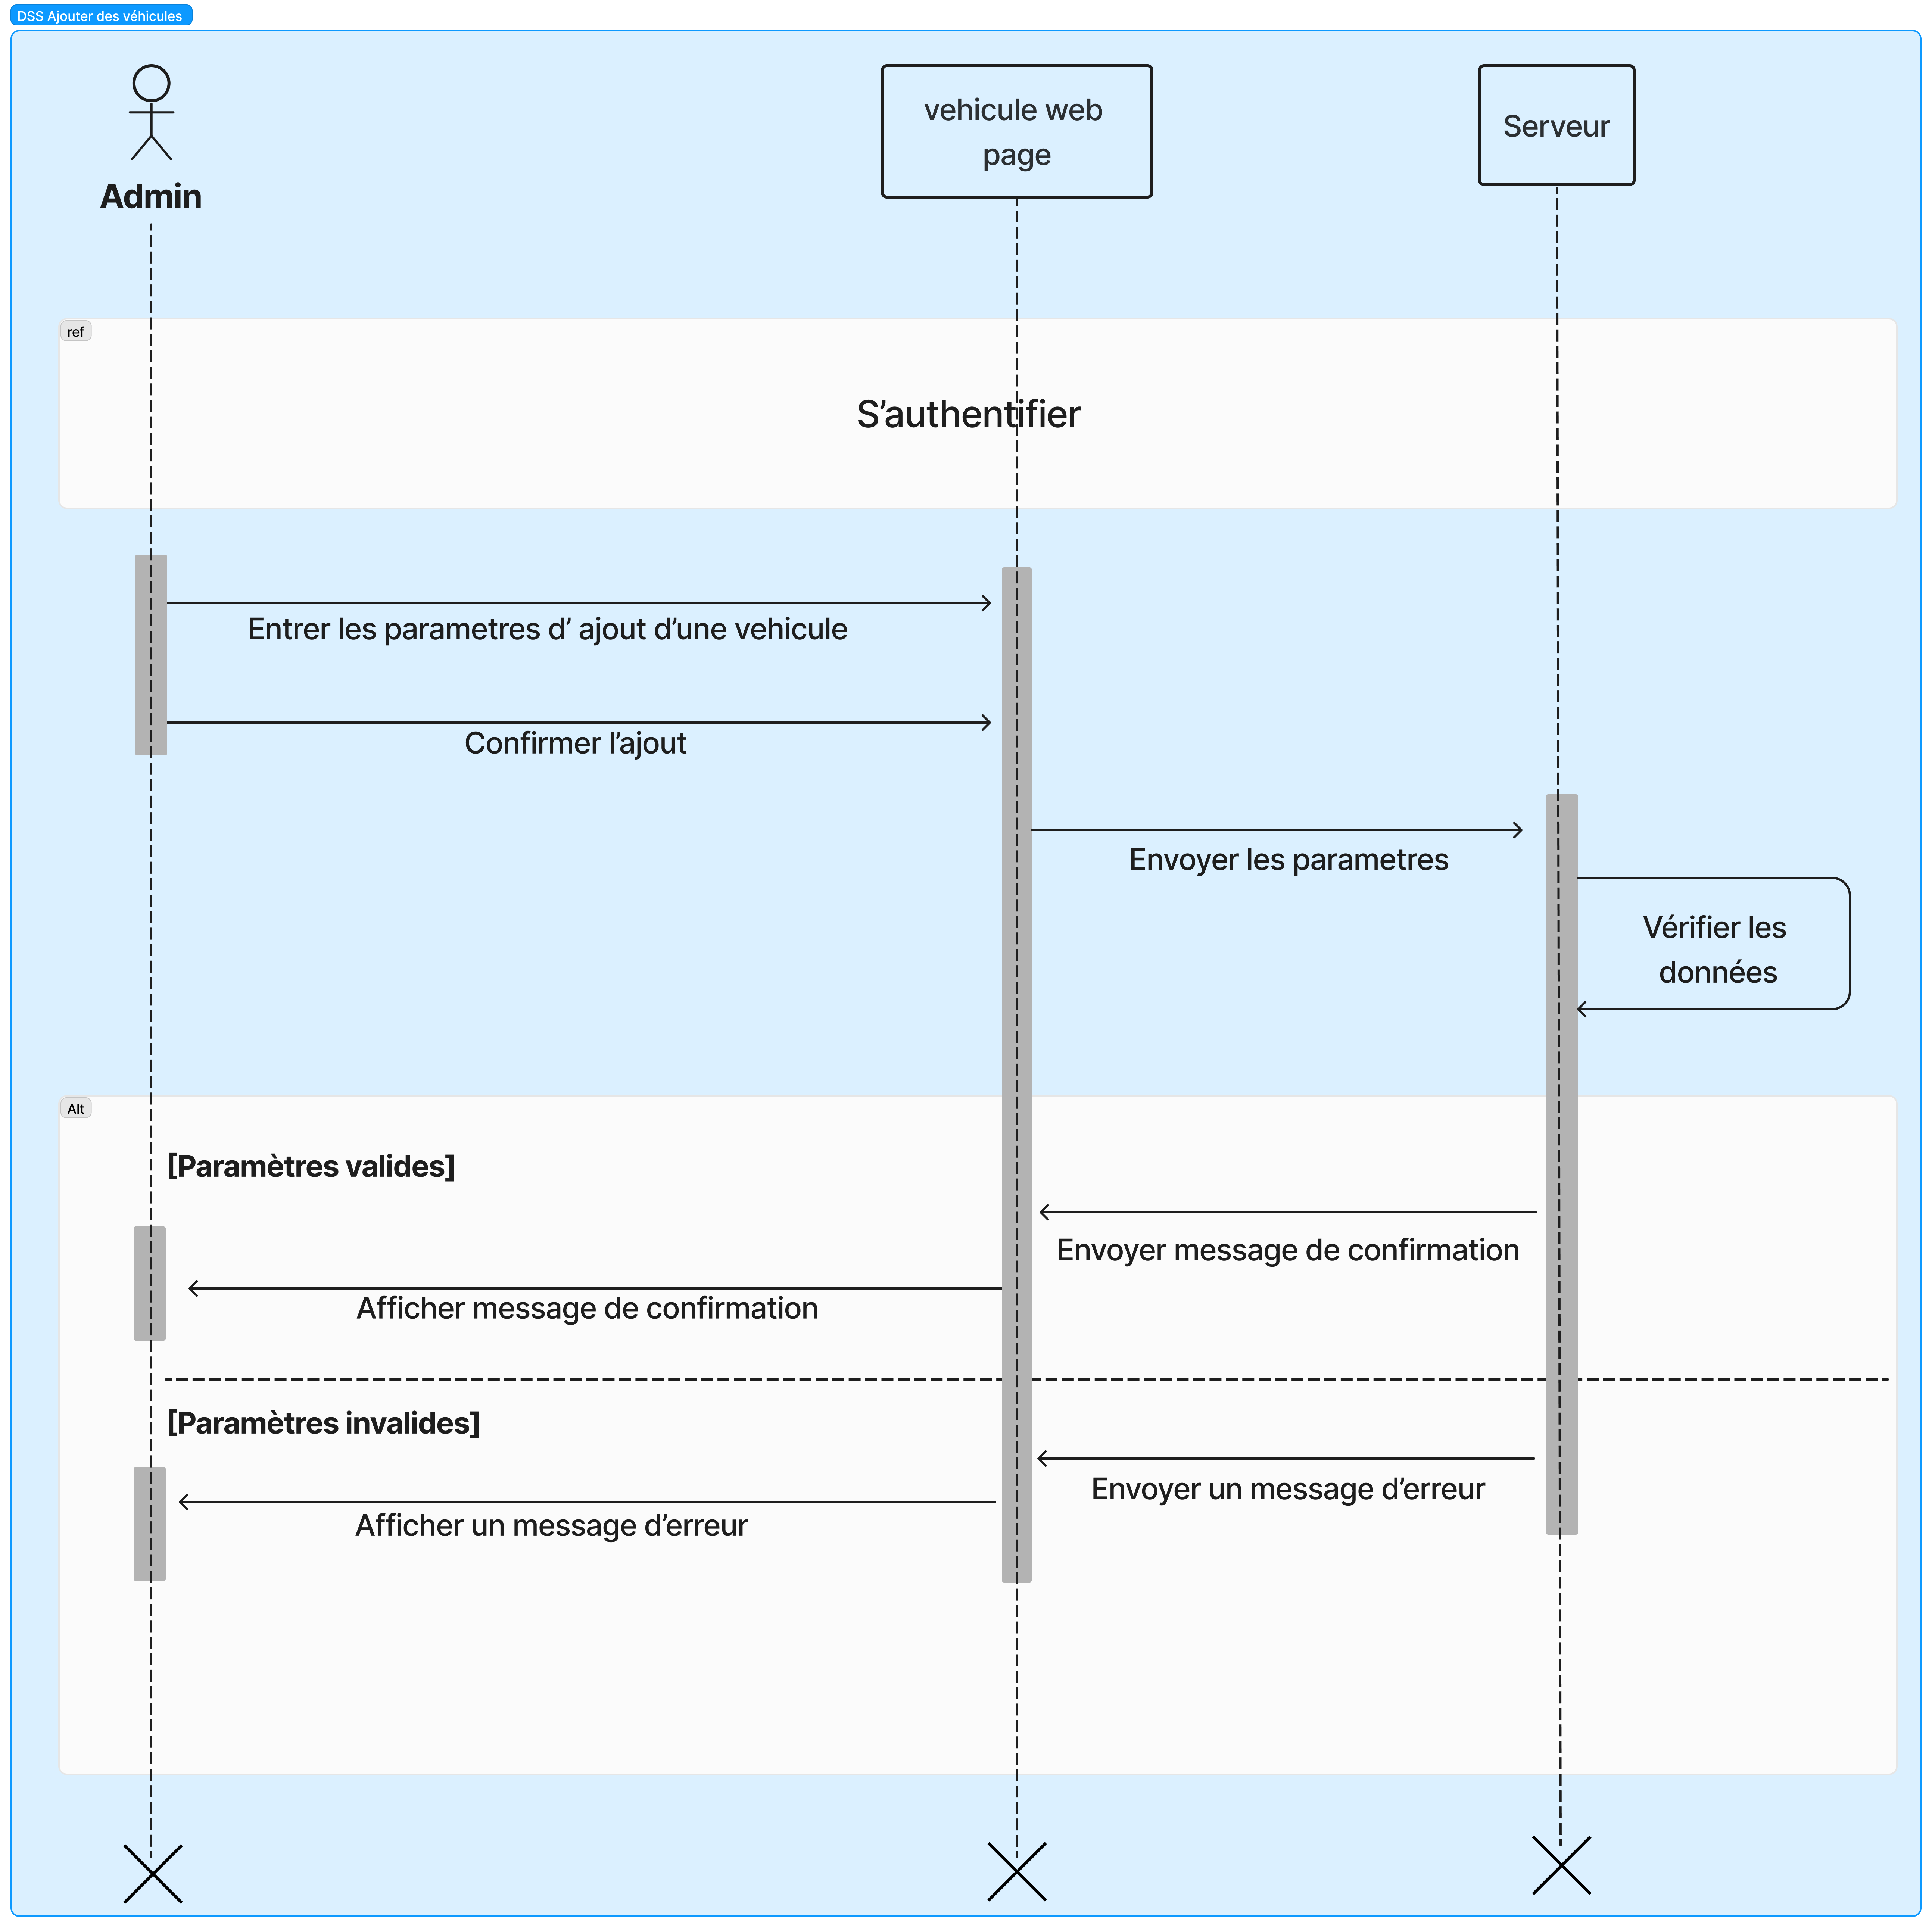
\includegraphics[width=1\textwidth,height=18cm]{chap4.images/dss ajouter vehicule.png}
  \caption{Raffinement de cas d’utilisation « Ajout des véhicules »}

\end{figure}


%________________________________________________________________________________________________________________
\newpage
\subsection{Raffinement du cas d'utilisation « Créer les taches »}

\begin{figure}[h!]
  \centering
  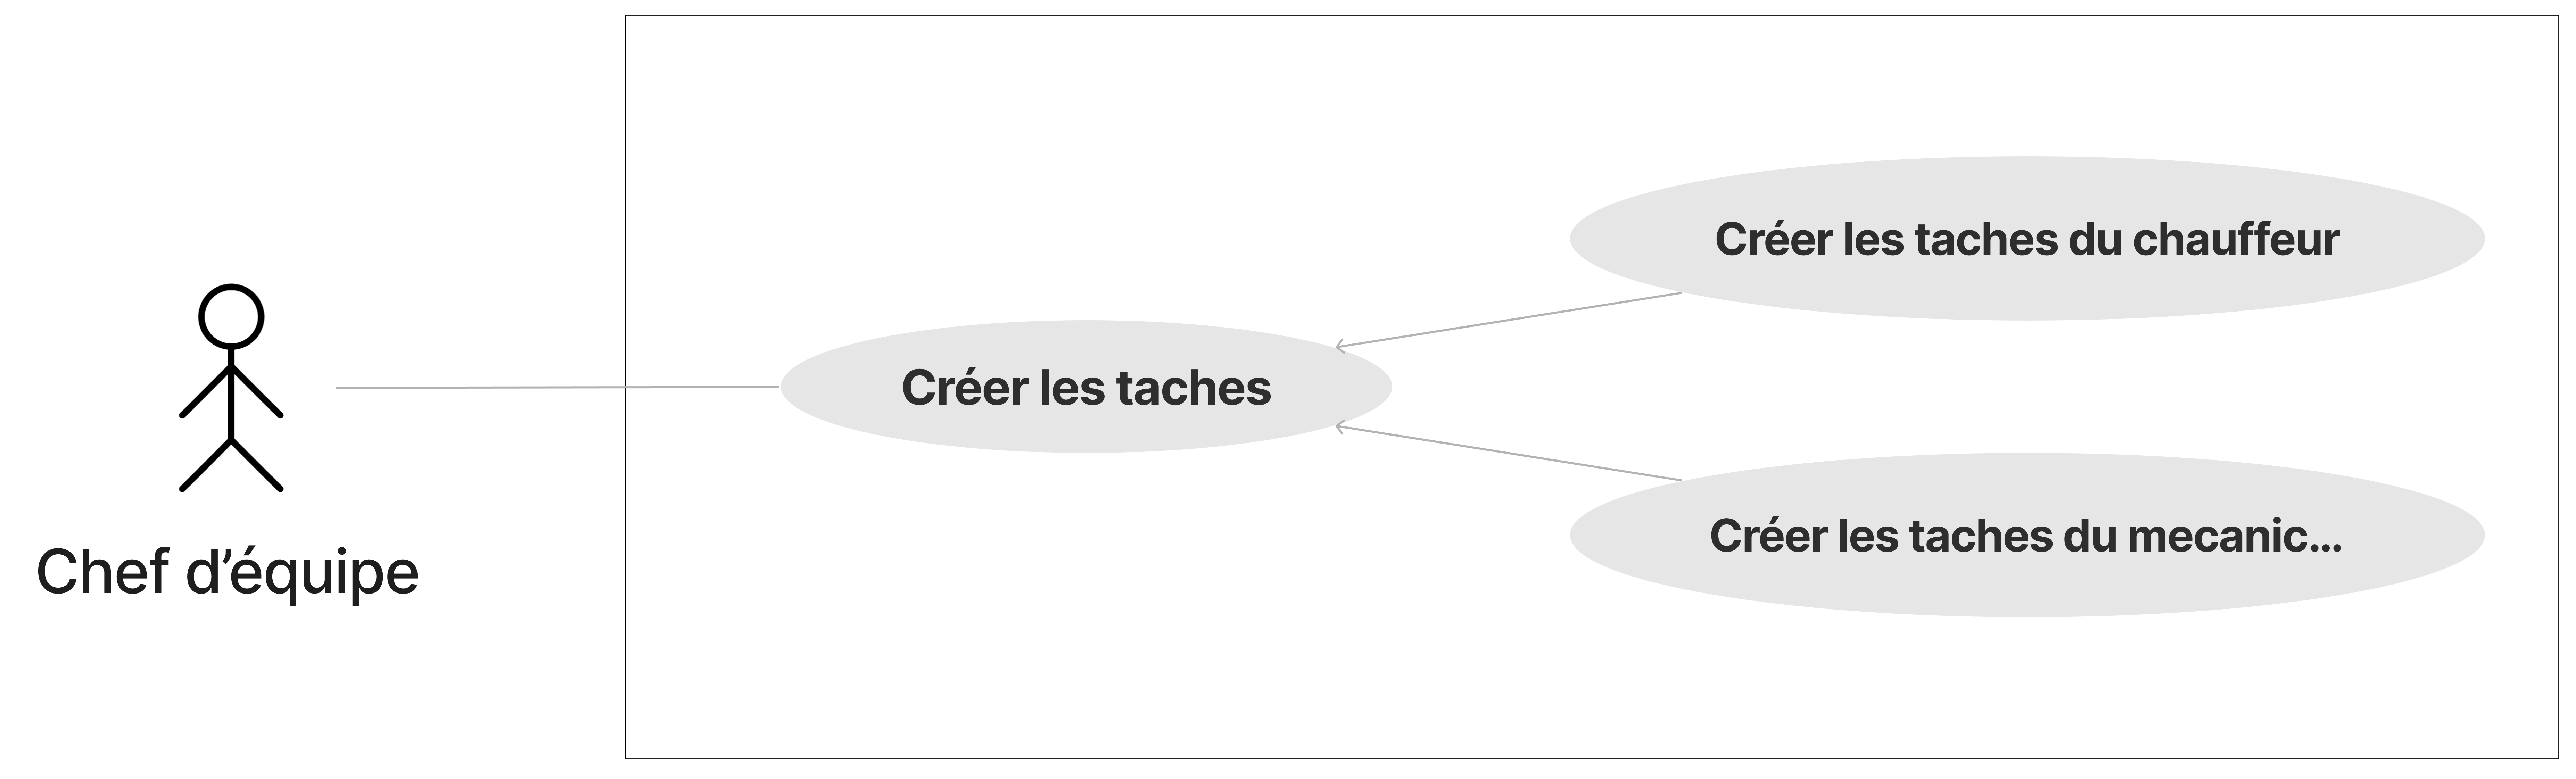
\includegraphics[width=1\textwidth,height=5cm]{chap4.images/raf creer taches.png}
  \caption{Raffinement de cas d’utilisation « Créer les taches »}

\end{figure}


%________________________________________________________________________________________________________________



\subsection{Description textuelle du cas d’utilisation « Créer des Tâches pour les Mécaniciens  »}

\begin{table}[H]
  \centering
  \renewcommand{\arraystretch}{1} % Facteur d'étirement des lignes
  \begin{tabular}{|p{4cm}|p{9cm}|}
    \hline
    \textbf{Cas d'utilisation} & Créer des Tâches pour les Mécaniciens                                                        \\
    \hline
    \textbf{Acteur}            & Chef d'Équipe                                                                                \\
    \hline
    \textbf{Pré-condition}     & 1-Le chef d'équipe est authentifié dans le système.\newline

    2-Il existe une liste de mécaniciens disponibles dans le système.                                                         \\
    \hline
    \textbf{Post-condition}    & Les tâches sont créées et assignées aux mécaniciens sélectionnés avec succès.                \\
    \hline
    \textbf{Scenario nominal}  & 1- Le chef d'équipe accède à l'interface de création de tâches pour les mécaniciens.\newline


    2- Le chef d'équipe choisit une date pour laquelle les tâches seront planifiées.\newline

    3-  Le système vérifie la disponibilité de cette date.\newline

    4- Le système affiche une liste des mécaniciens disponibles pour cette date.\newline

    5- Le chef d'équipe sélectionne un mécanicien parmi la liste pour lui assigner une tâche.\newline

    6- Le chef d'équipe saisit les détails de la tâche, y compris le titre, la description.                                   \\
  \end{tabular}

\end{table}


\begin{table}[H]
  \centering
  \renewcommand{\arraystretch}{1} % Facteur d'étirement des lignes
  \begin{tabular}{|p{4cm}|p{9cm}|}


                                 & 6- Le chef d'équipe confirme la création de la tâche et l'assignation du mécanicien.\newline

    7- Le système enregistre la tâche créée et envoie une notification au mécanicien assigné.                                   \\
    \hline
    \textbf{Scénario alternatif} & A1 Date non disponible \newline

    L’enchaînement A1 démarre au point 3 du scénario nominal.\newline

    4- un message d’erreur indiquant que pas de mécanicien disponible pour cette date.\newline

    Le scénario nominal reprend au point 2.                                                                                     \\


    \hline
  \end{tabular}
  \caption{Description textuelle du cas d’utilisation “Créer des Tâches pour les Mécaniciens ”}

\end{table}

\bigskip

\subsection{Description textuelle du cas d’utilisation « Créer des Tâches pour les Chauffeurs »}

\begin{table}[H]
  \centering
  \renewcommand{\arraystretch}{1.2}
  \begin{tabular}{|p{4cm}|p{9cm}|}
    \hline
    \textbf{Cas d'utilisation} & Créer des Tâches pour les Chauffeurs                                                              \\
    \hline
    \textbf{Acteur}            & Chef d'Équipe                                                                                     \\
    \hline
    \textbf{Pré-condition}     & 1- Le chef d'équipe est authentifié .\newline

    2- Les véhicules et les chauffeurs choisis sont disponibles dans le système.                                                   \\
    \hline
    \textbf{Post-condition}    & La tâche est correctement créée et assignée au chauffeur avec toutes les informations nécessaires \\
    \hline
    \textbf{Scenario nominal}  & 1- Le chef d'équipe accède à l'interface de création des tâches pour les chauffeurs.\newline


    2- Le chef sélectionne le modèle de véhicule souhaité pour la tâche.                                                           \\
  \end{tabular}
\end{table}


\begin{table}[H]
  \centering
  \renewcommand{\arraystretch}{1.1}
  \begin{tabular}{|p{4cm}|p{9cm}|}

                                 & 3- Le chef choisit la date pour laquelle la tâche est à planifier.\newline

    4- Le système affiche les véhicules disponibles qui correspondent au modèle sélectionné et sont libres à la date choisie.\newline

    5- Le chef d'équipe sélectionne un véhicule par sa matricule, puis saisit l'ID de la tâche et une description détaillée de celle-ci. \newline

    6- Le chef d’équipe recherche les chauffeurs qualifiés pour conduire le modèle de véhicule choisi et qui sont disponibles à la date spécifiée.\newline

    7- Le système vérifie les choix du chef d’équipe.\newline

    8- Le chef assigne la tâche à un chauffeur sélectionné et met à jour le QR code du véhicule pour refléter les détails de la nouvelle tâche.\newline

    9- Le système enregistre la tâche avec toutes les informations nécessaires et informe le chauffeur assigné. \\

    \hline
    \textbf{Scénario alternatif} & A1 Chauffeur qualifié non disponible \newline

    L’enchaînement A1 démarre au point 7 du scénario nominal.\newline

    4- un message d’erreur pour refaire le choix du chauffeur.\newline

    Le scénario nominal reprend au point 6.                                                                     \\


    \hline
  \end{tabular}
  \caption{Description textuelle du cas d’utilisation “Créer des Tâches pour les chauffeurs ”}

\end{table}



\newpage
\subsection{Diagramme de séquence système du cas d’utilisation «Créer les tâches pour les chauffeurs»}

\begin{figure}[ht!]
  \centering
  \includegraphics[width=1\textwidth,height=19cm]{chap4.images/dss créer taches des chauffeur.png}
  \caption{ Diagramme de séquence système du cas d’utilisation «Créer les tâches pour les chauffeurs» }
\end{figure}

%________________________________________________________________________________________________________________

\newpage
\subsection{Raffinement du cas d'utilisation « Consulter les taches pour les chauffeurs »}

\begin{figure}[h!]
  \centering
  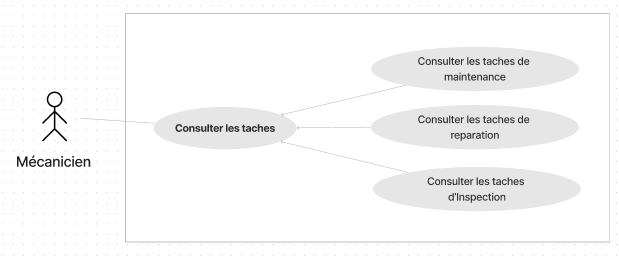
\includegraphics[width=0.9\textwidth,height=5cm]{chap4.images/raf consulter chauf.png}
  \caption{Analyse de cas d’utilisation « Consulter les taches pour les chauffeurs »}

\end{figure}

\subsection{Description textuelle du cas d’utilisation « Consulter les taches pour les chauffeurs »}

\begin{table}[H]
  \centering
  \renewcommand{\arraystretch}{1} % Facteur d'étirement des lignes
  \begin{tabular}{|p{4cm}|p{9cm}|}
    \hline
    \textbf{Cas d'utilisation}    & Consulter les taches des chauffeurs                                                                                 \\
    \hline
    \textbf{Acteur Principal }    & Chauffeur                                                                                                           \\
    \hline
    \textbf{Acteurs Secondaires } & Chef d’Équipe                                                                                                       \\
    \hline
    \textbf{Pré-condition}        & 1- Le chauffeur doit être connecté à l'application .\newline

    2-  Des tâches doivent être assignées au chauffeur.                                                                                                 \\
    \hline
    \textbf{Post-condition}       & 1- Le chauffeur a consulté les détails de ses tâches.\newline

    2- Le chauffeur peut confirmer la réalisation des tâches.\newline

    3- Le chef d’équipe est informé de l’avancement ou de l’achèvement des tâches.                                                                      \\

    \hline
    \textbf{Scenario nominal}     & 1- Lorsqu’une nouvelle tâche est assignée, le chauffeur reçoit une notification sur son application mobile.
    \newline


    2- Le chauffeur est invité à scanner un code QR pour accéder à sa checklist quotidienne.\newline

    3- Le système affiche la checklist quotidienne du chauffeur, comprenant toutes les tâches assignées avec des détails spécifiques pour chaque tâche. \\
  \end{tabular}

\end{table}

\begin{table}[htbp]
  \centering
  \renewcommand{\arraystretch}{1.7} % Facteur d'étirement des lignes
  \begin{tabular}{|p{4cm}|p{9cm}|}

                                 & 4- Une fois qu’une tâche est accomplie, le chauffeur confirme sa réalisation directement depuis l’application en marquant la tâche comme "Terminée". \newline

    5- Le système notifie automatiquement le chef d’équipe de l’avancement ou de l’achèvement des tâches confirmées par le chauffeur.                                                            \\


    \hline
    \textbf{Scénario alternatif} & A1 Absence de Checklist \newline

    L'enchainement démarre au point 3 du scénario nominal.\newline

    4- Un message d'erreur s'affiche pour réaccéder à la checklist. \newline

    Le scénario reprend au point 2.                                                                                                                                                              \\                                                                                                                                                        

    \hline
  \end{tabular}
  \caption{Description textuelle du cas d’utilisation “Consulter les taches des chauffeurs”}

\end{table}


\newpage
\subsection{Diagramme d'activité du cas d’utilisation «Consulter les taches des chauffeurs» }

\begin{figure}[ht!]
  \centering
  \includegraphics[width=0.9\textwidth,height=10cm]{chap4.images/taches activité.png}
  \caption{ Diagramme d'activité du cas d’utilisation « Consulter les taches des chauffeurs » }
\end{figure}


%________________________________________________________________________________________________________________
%________________________________________________________________________________________________________________

\newpage
\subsection{Raffinement du cas d'utilisation « Consulter les taches pour les mécaniciens »}
\begin{figure}[h!]
  \centering
  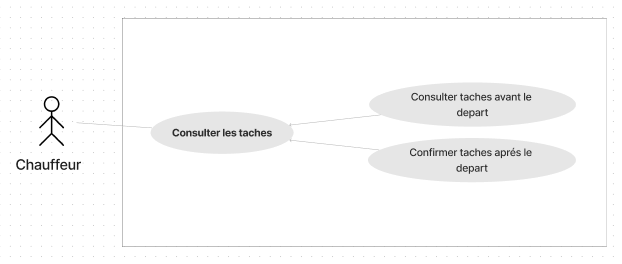
\includegraphics[width=0.9\textwidth,height=5cm]{chap4.images/raf consulter mec.png}
  \caption{Analyse de cas d’utilisation « Consulter les taches pour les mécaniciens »}

\end{figure}

\subsection{Description textuelle du cas d’utilisation « Consulter les taches pour les mécaniciens »}

\begin{table}[htbp]
  \centering
  \renewcommand{\arraystretch}{1.7} % Facteur d'étirement des lignes
  \begin{tabular}{|p{4cm}|p{9cm}|}
    \hline
    \textbf{Cas d'utilisation}    & Consulter les tâches des  mécaniciens                                                                                            \\
    \hline
    \textbf{Acteur Principal}     & Mécanicien                                                                                                                       \\
    \hline
    \textbf{Acteurs Secondaires } & Chef d’Équipe                                                                                                                    \\
    \hline
    \textbf{Pré-condition}        & 1- Le mécanicien doit être authentifié dans le système.\newline

    2- Des tâches doivent être assignées au mécanicien.                                                                                                              \\
    \hline
    \textbf{Post-condition}       & 1- Le mécanicien est informé des nouvelles tâches.\newline

    2- Les tâches sont consultées et confirmées une fois réalisées.             \newline

    3- Le chef d’atelier est notifié de la réalisation des tâches.                                                                                                   \\

    \hline
    \textbf{Scenario nominal}     & 1- Le mécanicien reçoit une notification sur son appareil mobile lui indiquant qu'une nouvelle tâche lui a été assignée.\newline


    2- Il accède à la liste des tâches disponibles.\newline

    3- Après avoir pris connaissance des détails, le mécanicien se met au travail pour effectuer la tâche.                                                           \\
  \end{tabular}

\end{table}


\begin{table}[htbp]
  \centering
  \renewcommand{\arraystretch}{1.7} % Facteur d'étirement des lignes
  \begin{tabular}{|p{4cm}|p{9cm}|}

                                 & 4- Une fois la tâche terminée, il marque la tâche comme réalisée dans l'application.\newline

    5- Le système envoie automatiquement une notification à son chef pour l'informer de l'achèvement de la tâche.\newline

    6- Le chef vérifie la réalisation de la tâche dans le système et valide l'achèvement.                                       \\


    \hline
    \textbf{Scénario alternatif} & A1 Absence de taches \newline

    L'enchainement démarre au point 3 du scénario nominal.\newline

    4- Un message d'erreur s'affiche pour réaccéder à la checklist. \newline

    Le scénario reprend au point 2.                                                                                             \\                                                                                           

    \hline
  \end{tabular}
  \caption{Description textuelle du cas d’utilisation “Consulter les tâches des mécaniciens”}

\end{table}

%________________________________________________________________________________________________________________



\newpage
\section{Diagramme de classes du sprint 2}

\begin{figure}[ht!]
  \centering
  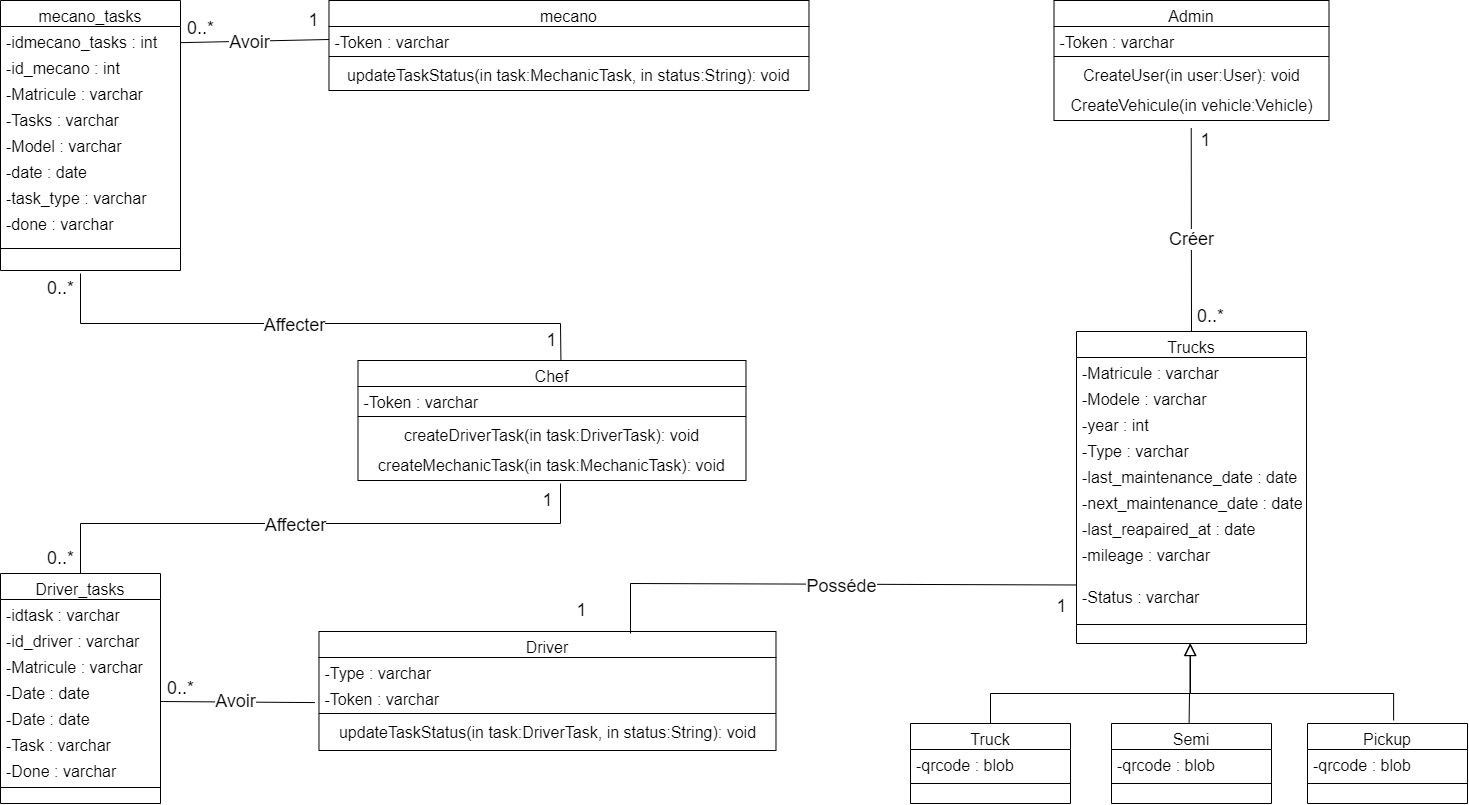
\includegraphics[width=1.1\textwidth,height=11cm]{chap4.images/class sprint 2.png}
  \caption{Diagramme de classes du sprint 2}

\end{figure}

%________________________________________________________________________________________________________________
\newpage
\section{ Réalisation}

Dans cette section, nous présentons les avancées réalisées durant le sprint 2. À travers des captures d’écran et des descriptions détaillées, nous illustrons les nouvelles fonctionnalités intégrées et les améliorations apportées aux interfaces existantes.

%%%%%%%%%%%%%%%%%%%%%%%%%%%%%%%%%%%%%%%%%

\subsection{Interface de création des taches}

Cette interface permet au chef d'équipe de créer des tâches pour les chauffeurs et les mécaniciens. Le chef d'équipe peut choisir le type de tâche à créer en sélectionnant soit une tâche pour un chauffeur, soit une tâche pour un mécanicien.

\begin{figure}[h!]
  \centering
  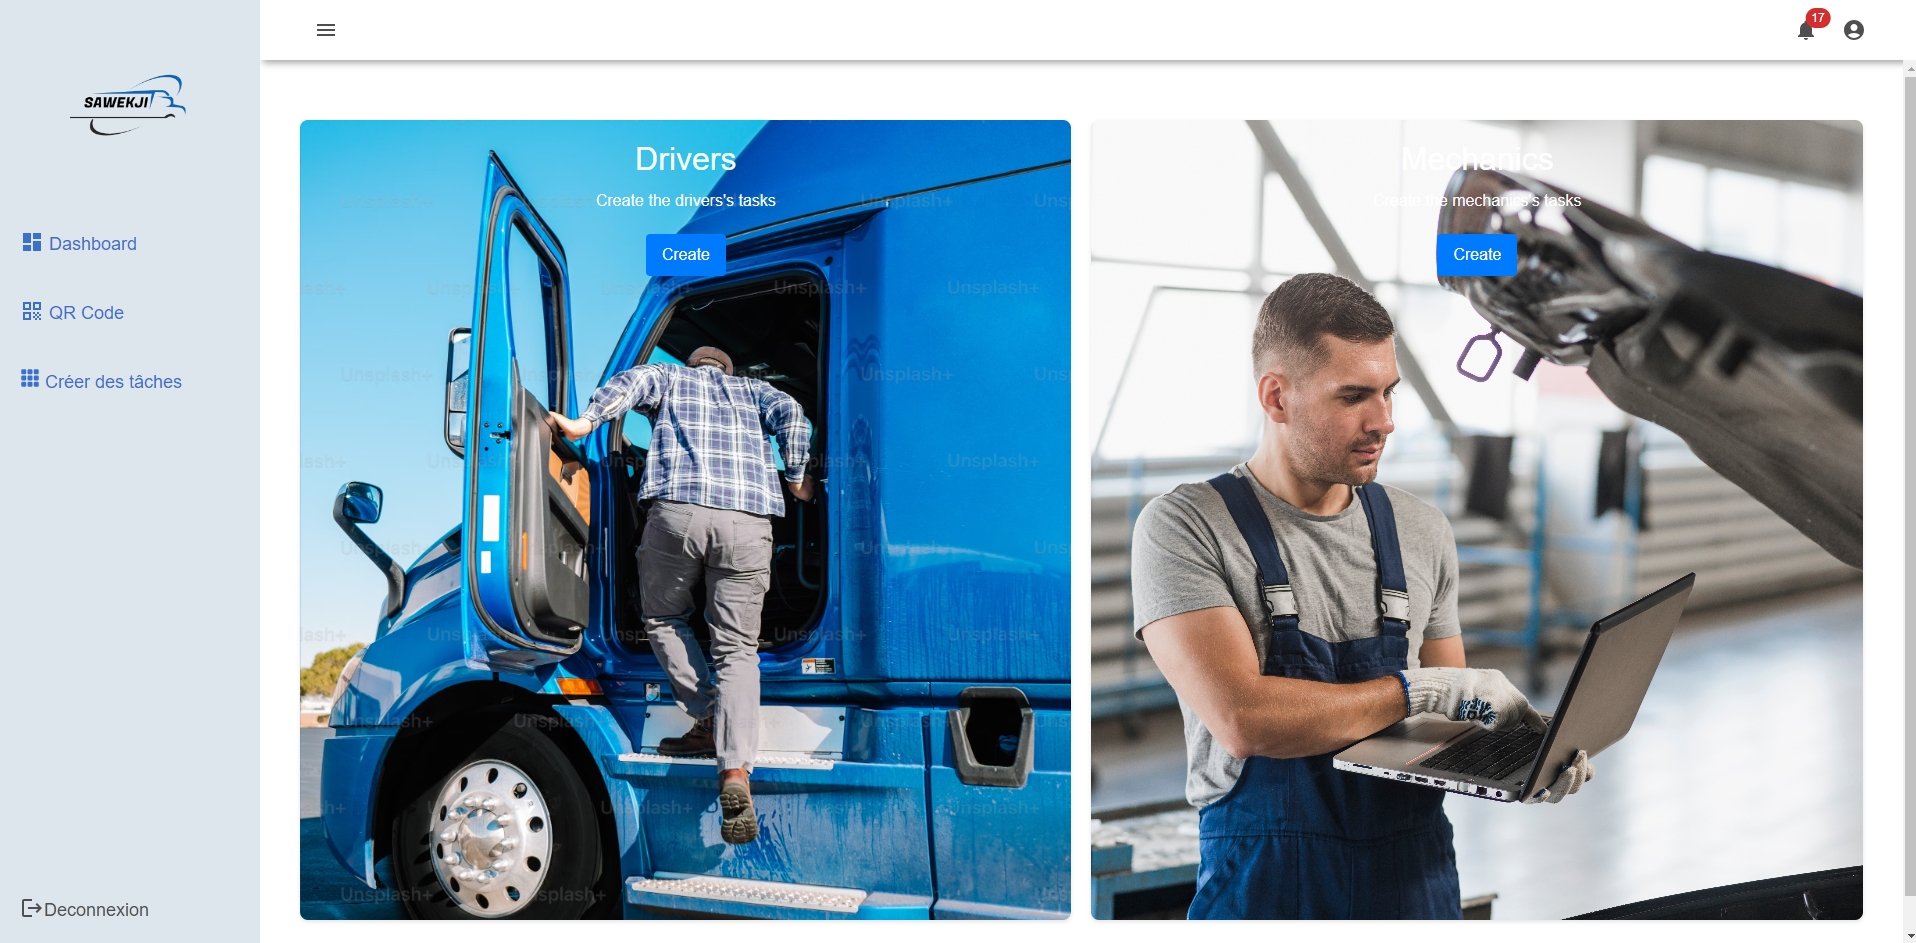
\includegraphics[width=0.9\textwidth,height=6.5cm]{chap4.images/creer taches.png}
  \caption{interface de création des taches}

\end{figure}


%%%%%%%%%%%%%%%%%%%%%%%%%%%%%%%%%%%%%%%%%

Cette interface permet au chef d'équipe de créer des tâches spécifiques pour les chauffeurs. Le processus inclut la sélection du modèle de voiture, la date de la tâche, une description détaillée de la tâche, et enfin, l'assignation de la tâche à un chauffeur spécifique. Cette capture d'écran montre les différentes options et champs à remplir pour une création de tâche complète et précise

\begin{figure}[h!]
  \centering
  \includegraphics[width=0.9\textwidth,height=6.5cm]{chap4.images/Création des taches mec.png}
  \caption{Création des taches pour les chauffeurs}

  \newpage
\end{figure}
\bigskip
Cette interface est dédiée à la création de tâches pour les mécaniciens. Le chef d'équipe peut sélectionner la date de la tâche, puis visualiser la liste des mécaniciens disponibles pour cette date. Ensuite, il peut assigner la tâche à un mécanicien particulier. Cette capture d'écran met en évidence les étapes de sélection et d'assignation, offrant une vue claire et fonctionnelle pour la gestion des interventions mécaniques.
\begin{figure}[h!]
  \centering
  \includegraphics[width=0.9\textwidth]{chap4.images/Création des taches chauff.png}
  \caption{Création des taches pour les mécaniciens}

\end{figure}
%________________________________________________________________________________________________________________

\subsection{Consultation du checklist du chauffeur}

\begin{figure}[htbp]
  \centering
  \begin{minipage}{0.58\textwidth}
    \raggedright
    Cette interface mobile permet aux chauffeurs de consulter leurs tâches assignées. Lorsqu'une nouvelle tâche est créée, le chauffeur reçoit une notification et est invité à scanner un code QR pour accéder à sa checklist quotidienne. Cette checklist comprend toutes les tâches à accomplir, avec des détails spécifiques pour chaque tâche. Le chauffeur peut alors confirmer la réalisation des tâches directement depuis l'application, ce qui notifie automatiquement le chef d'équipe de l'avancement ou de l'achèvement des tâches.
  \end{minipage}
  \hfill
  \begin{minipage}{0.39\textwidth}
    \centering
    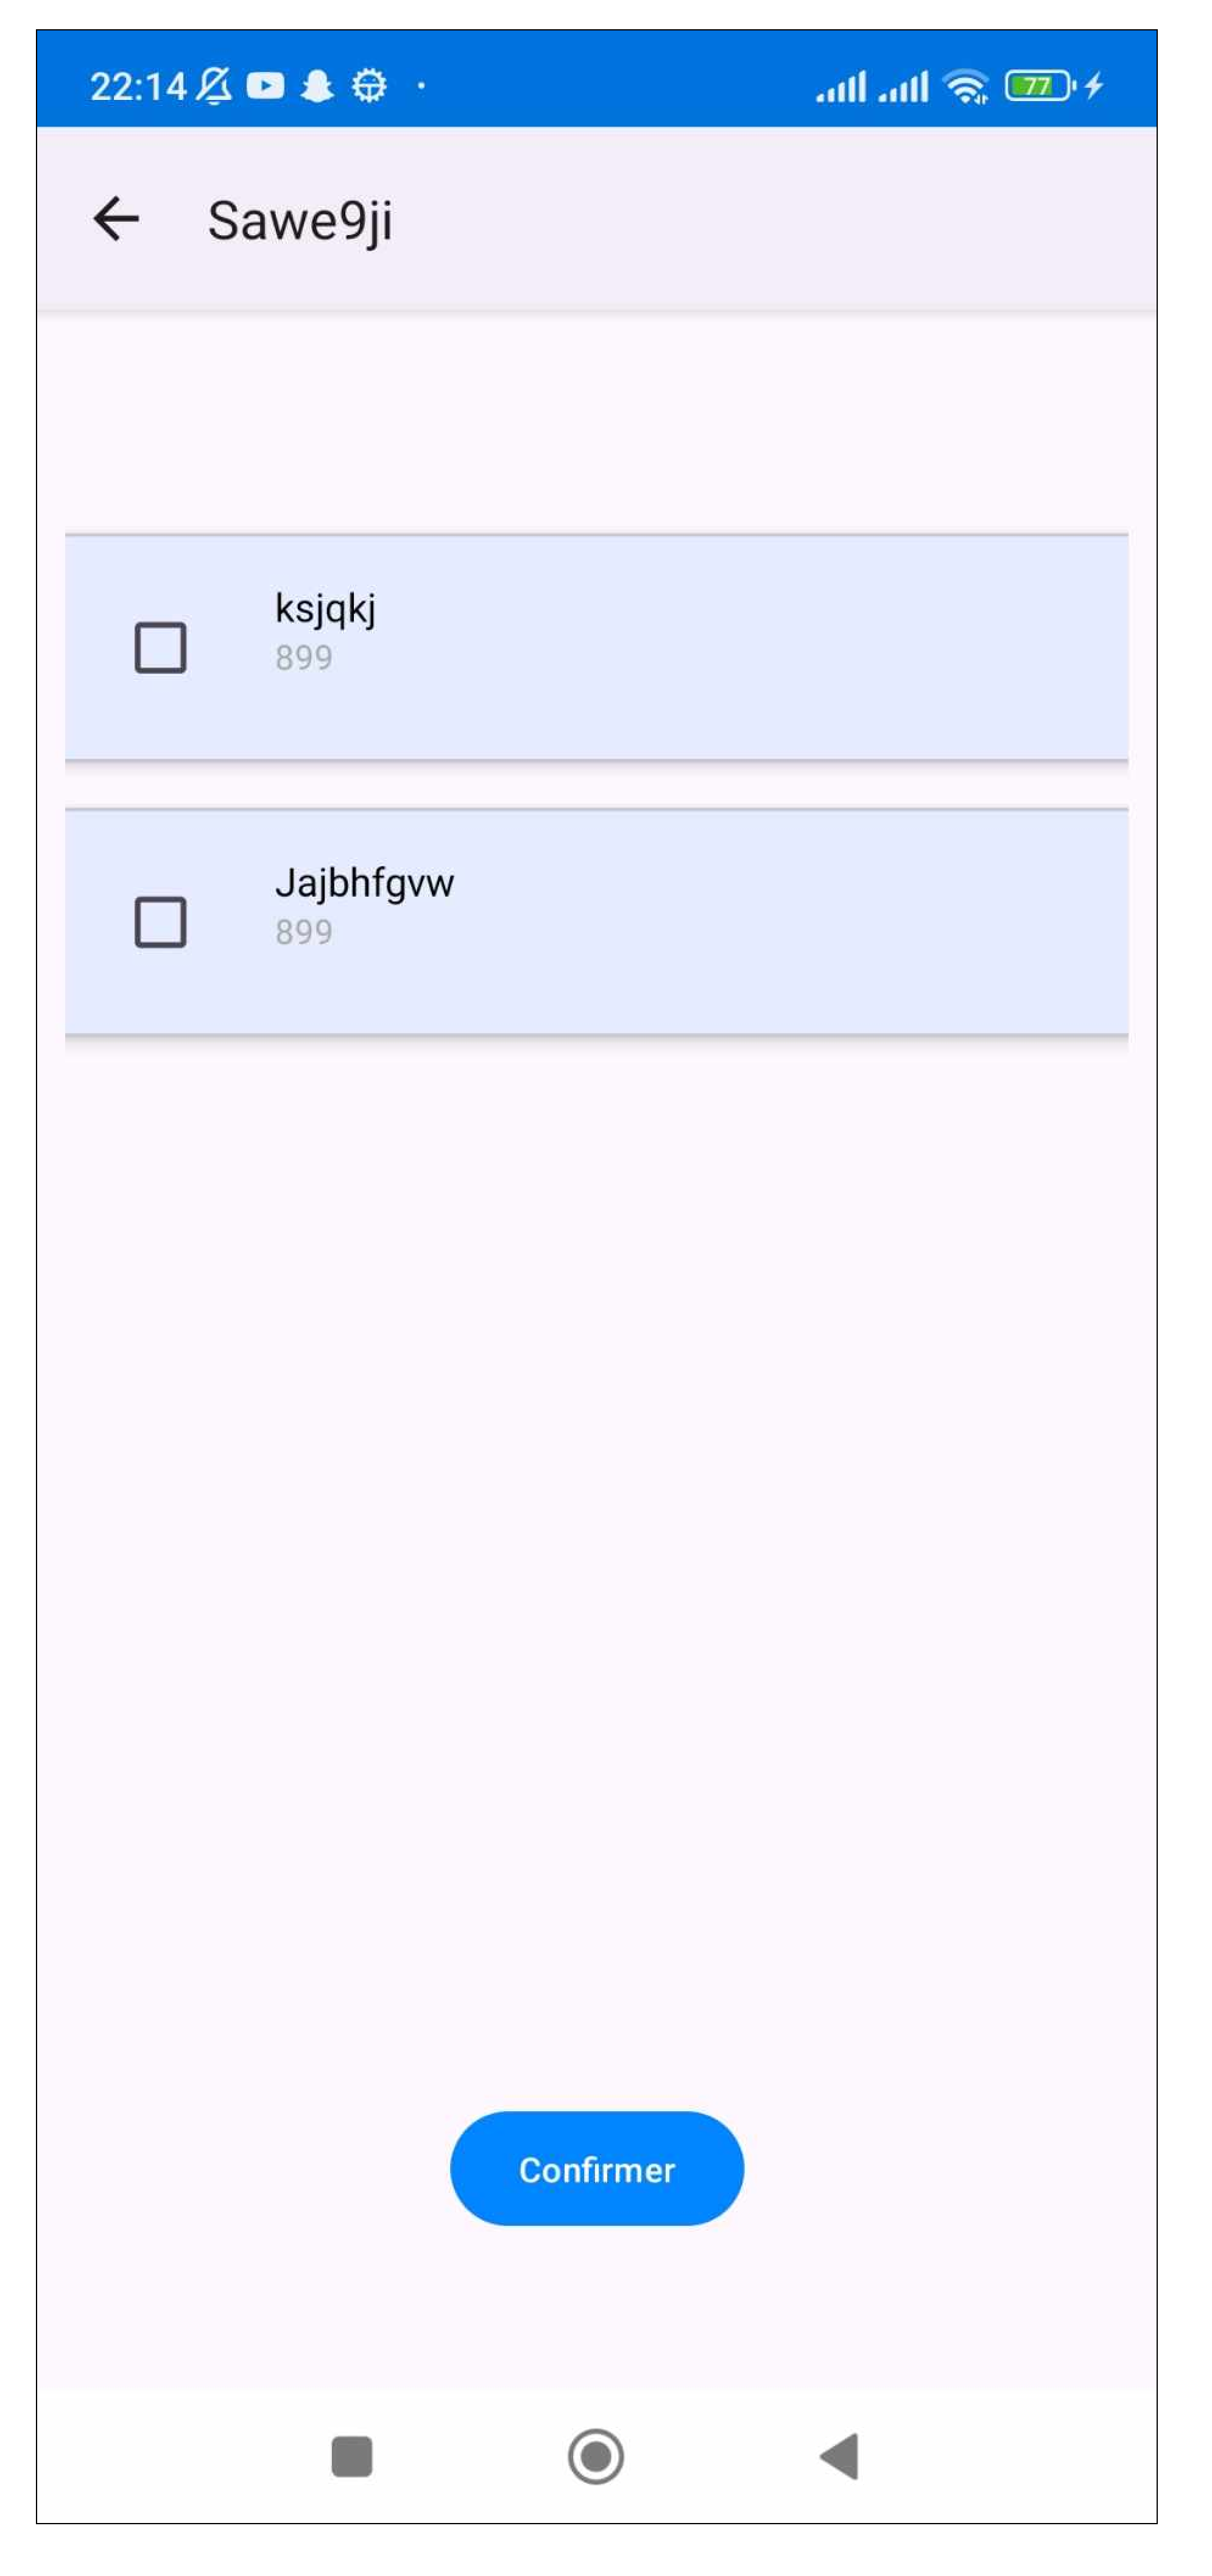
\includegraphics[width=0.8\textwidth,height=8cm]{chap4.images/consultation du checklist.png}
    \caption{interface de consultation du checklist pour les chauffeurs }
  \end{minipage}
\end{figure}

\newpage

\subsection{Consulation des taches du mécanicien }

\begin{figure}[htbp]
  \centering
  \begin{minipage}{0.58\textwidth}
    \raggedright
    Cette interface mobile est destinée aux mécaniciens pour la gestion de leurs tâches assignées. À chaque nouvelle tâche, le mécanicien reçoit une notification l'invitant à consulter les détails de la tâche sur l'application. L'interface affiche les nouvelles tâches avec les informations nécessaires. Le mécanicien peut alors confirmer la réalisation de chaque tâche, ce qui envoie une notification au chef d'équipe pour informer de l'état d'avancement.
  \end{minipage}
  \hfill
  \begin{minipage}{0.39\textwidth}
    \centering
    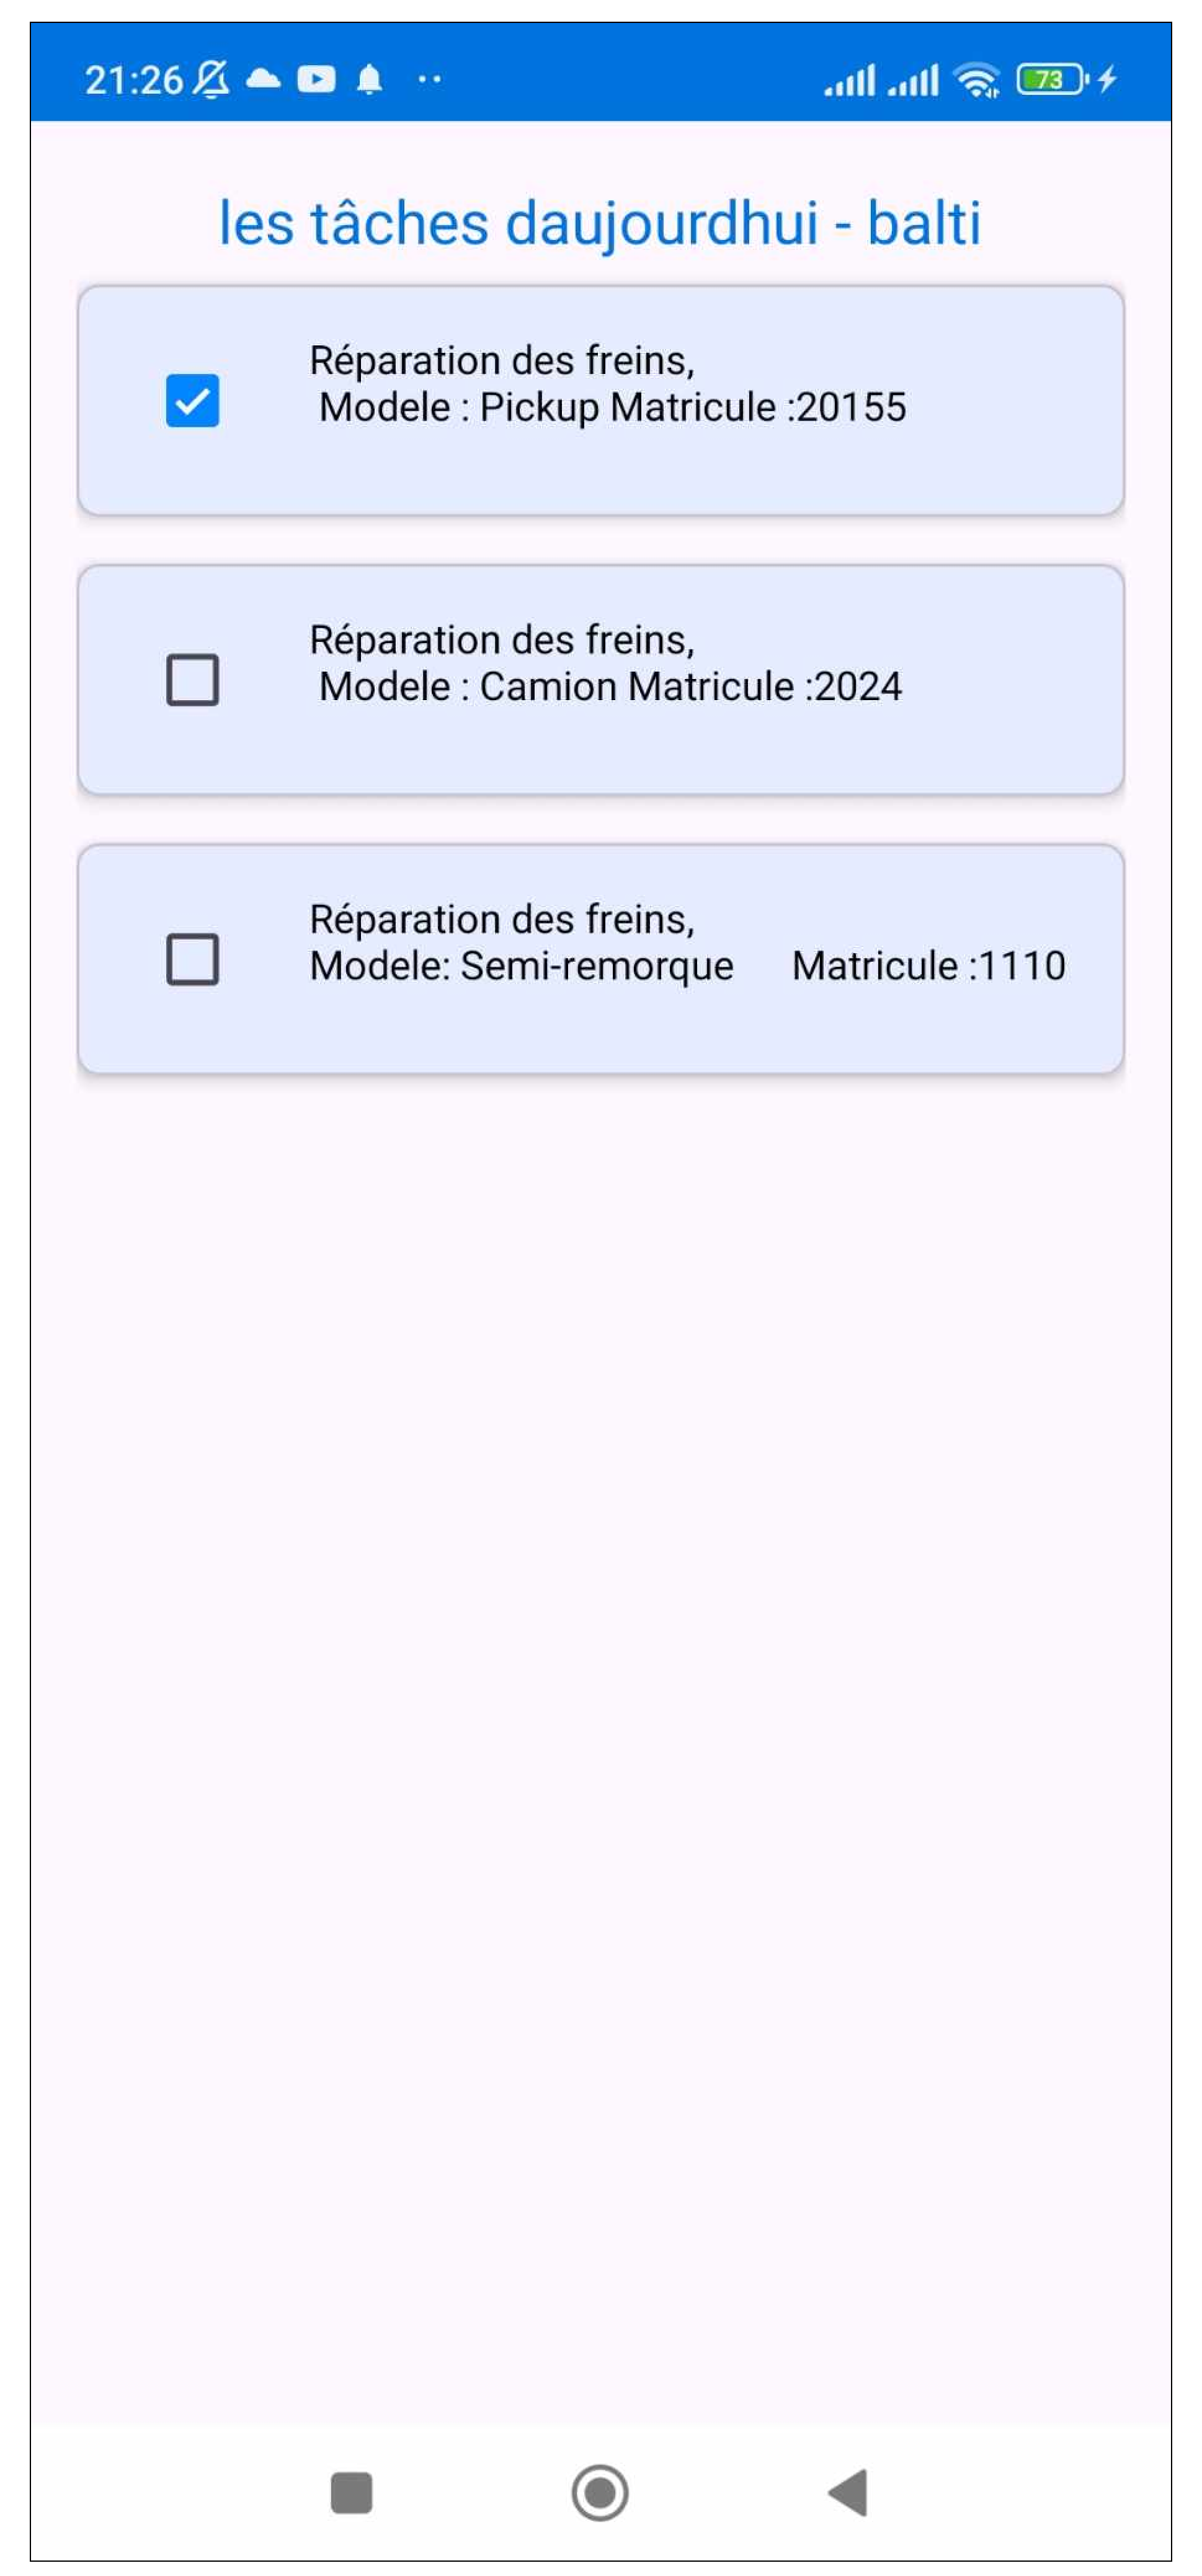
\includegraphics[width=0.8\textwidth,height=7.5cm]{chap4.images/consulation des taches.png}
    \caption{interface de consulation des taches pour les mécaniciens }
  \end{minipage}
\end{figure}
\bigskip
\subsection{Validation des taches du mécanicien par le chef d'équipe }

\begin{figure}[htbp]
  \centering
  \begin{minipage}{0.58\textwidth}
    \raggedright
    Cette interface permet au chef d'équipe de confirmer les tâches effectuées par les mécaniciens. Elle affiche une liste des tâches en attente de validation. Chaque tâche est présentée  par ca description et Le nom du mécanicien responsable de la tâche.\\

    Le chauffeur, après avoir vérifié sur le terrain l'accomplissement de la tâche, il peut confirmer la tâche en appuyant sur le bouton "Confirm Tache" correspondant.
  \end{minipage}
  \hfill
  \begin{minipage}{0.39\textwidth}
    \centering
    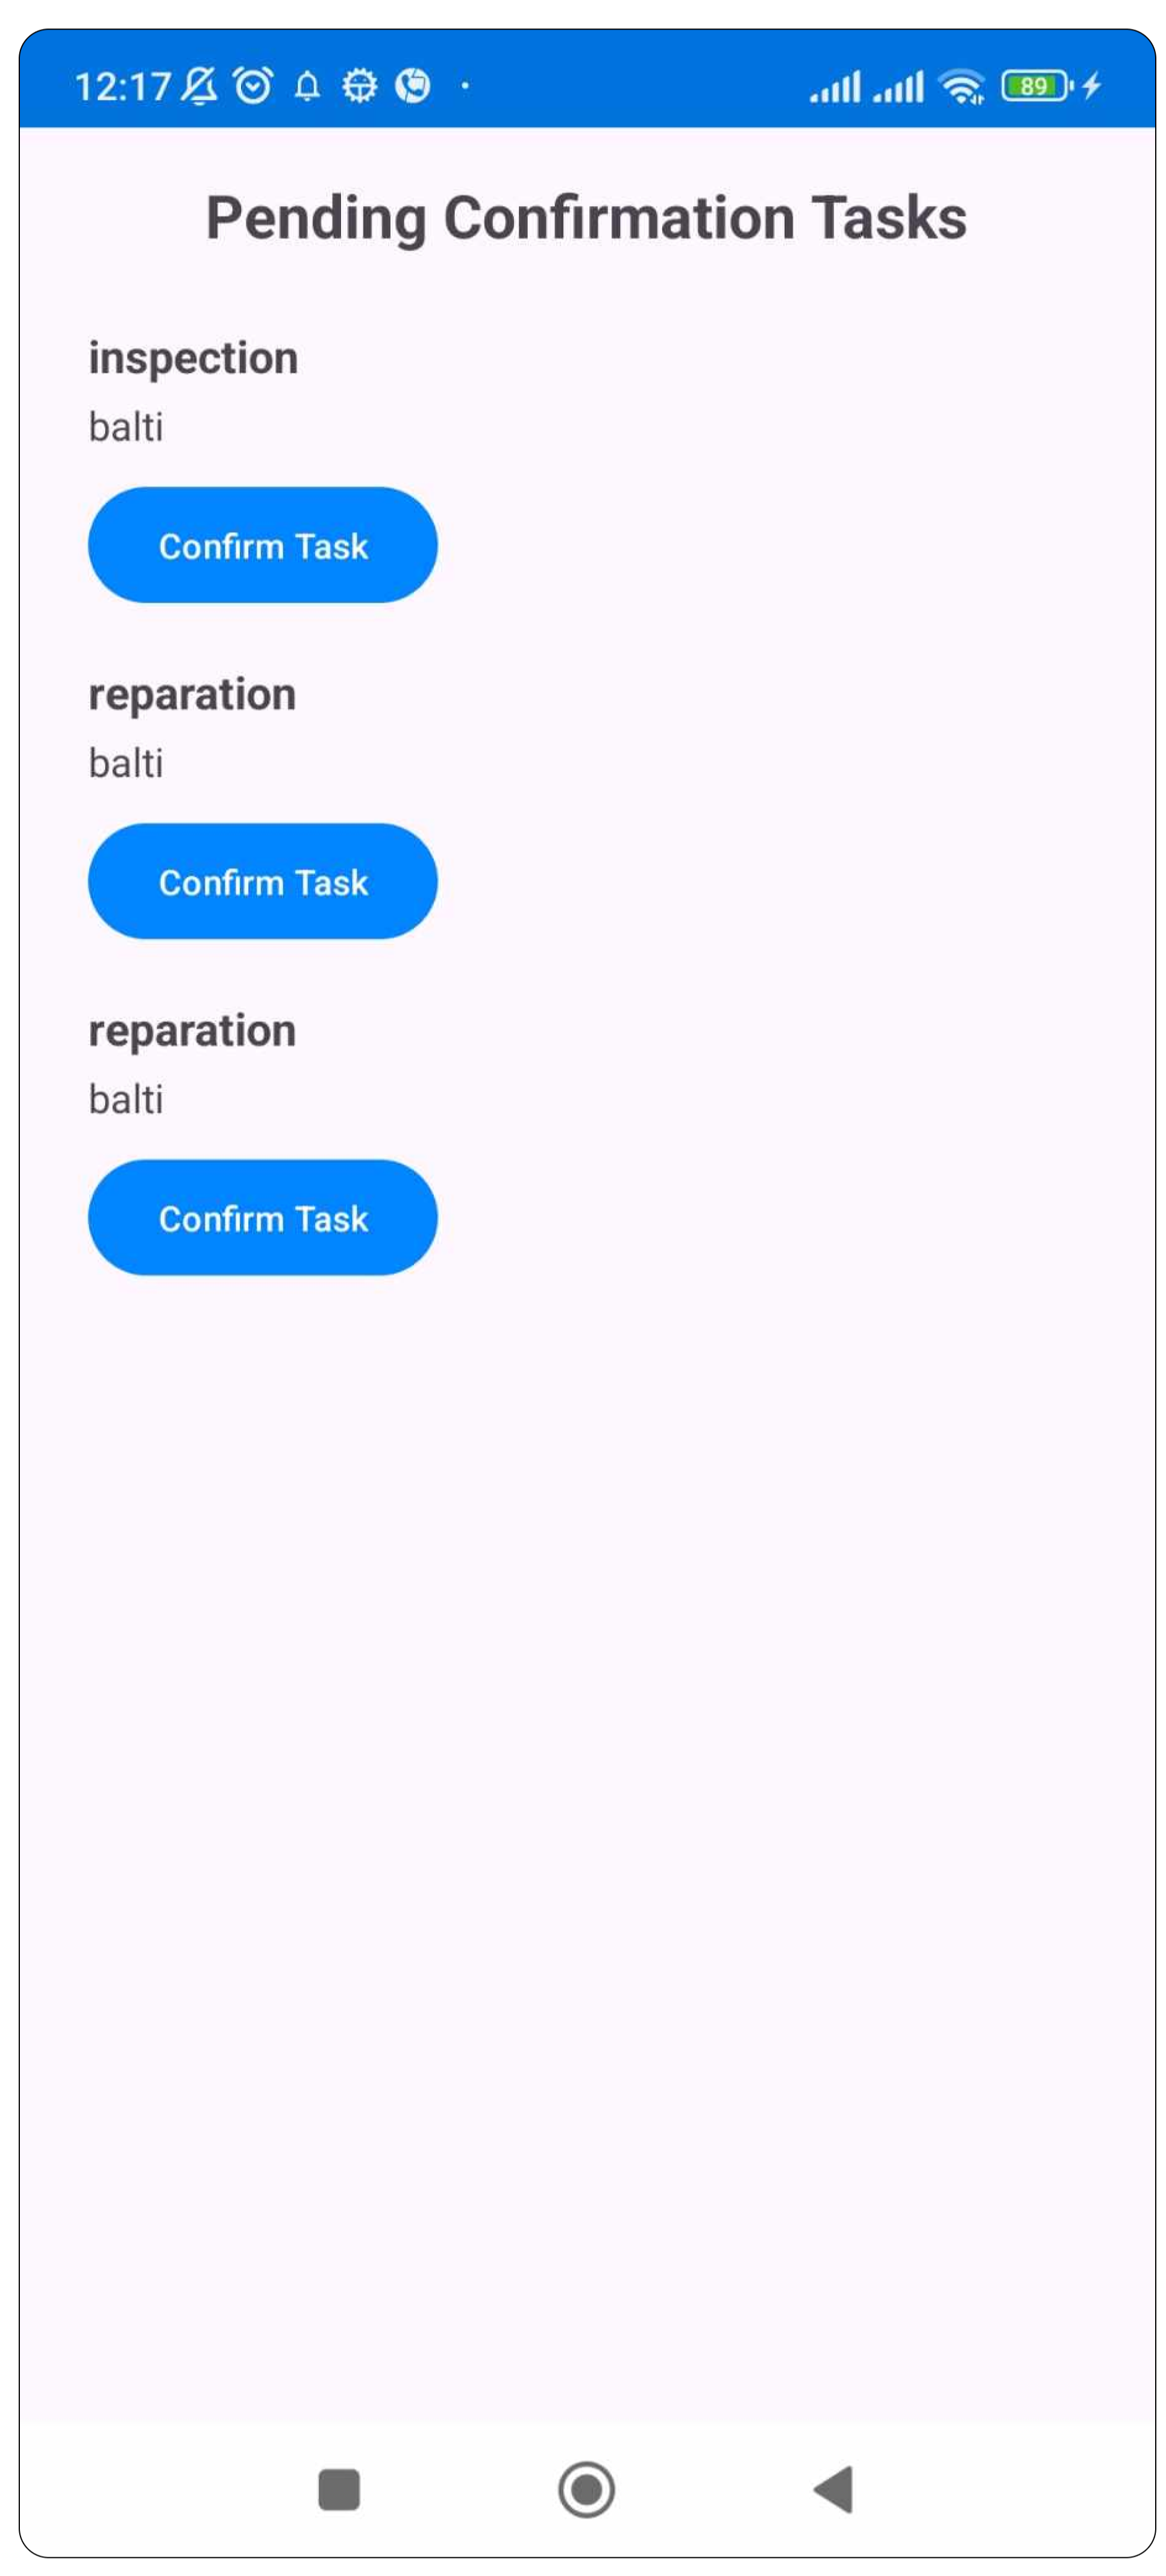
\includegraphics[width=0.8\textwidth,height=7.5cm]{chap4.images/valider taches.png}
    \caption{interface de consulation des taches pour les mécaniciens }
  \end{minipage}
\end{figure}


%________________________________________________________________________________________________________________

\newpage
\section{Rétrospective}
Dans cette rétrospective du Sprint 2, nous évaluerons les performances de notre équipe en utilisant le burndown chart et le task board. Ces outils nous aident à identifier les succès, les défis rencontrés, et les possibilités d'amélioration pour les prochains sprints.

\subsection{Burdown Chart}
Nous avons planifié un sprint de 3 semaines, avec une moyenne de 6 heures de travail par jour.


\begin{figure}[h!]
  \centering
  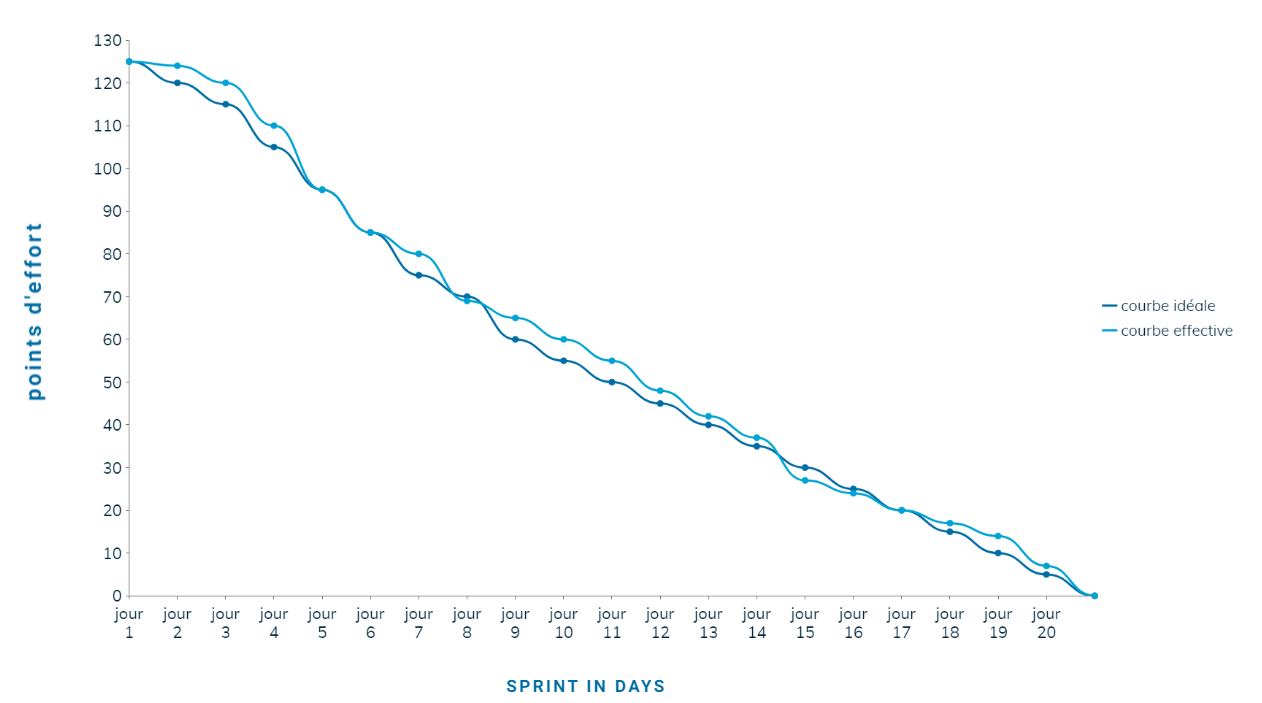
\includegraphics[width=1\textwidth, height=6.7cm]{chap4.images/Burndown chart sprint 2.png}
  \caption{ Burdown Chart du Sprint 2}

\end{figure}
%%%%%%%%%%%%%%%%%%%%%%%%%%%%%%%%%%%%%%%%%
\subsection{Task Bord}

La figure 4.14 présente le "Task Bord" correspondant au 9ème jour du sprint 2.

\begin{figure}[h!]
  \centering
  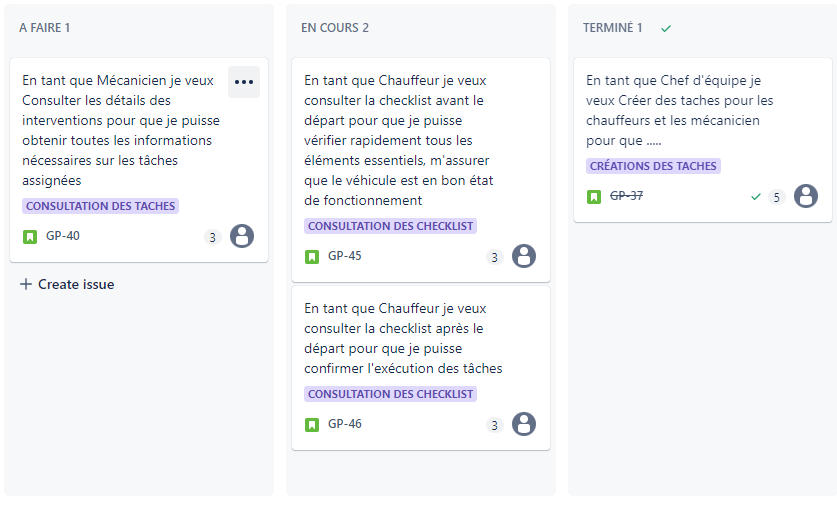
\includegraphics[width=0.9\textwidth, height=6.7cm]{chap4.images/task board sprint 2.png}
  \caption{ Task board du Sprint 2 }

\end{figure}

%_______________________________________________________________________________________________
\newpage
\section{tests unitaires}
\textbf{Test unitaires du cas d’utilisation « Créer taches  » :}\\
\bigskip
Nous présentons ci-dessous le code source et le résultat de deux cas de test :
\bigskip


\textbf{1. Test de réussite :} Le test est considéré comme réussi lorsque le chef d'équipe crée des tâches en utilisant des ID valides existants.

\textbf{2. Test d'échec :} Le test est considéré comme échoué si le chef d'équipe tente d'utiliser un ID inexistant lors de la création d'une nouvelle tâche.

\bigskip

\begin{figure}[h!]
  \centering
  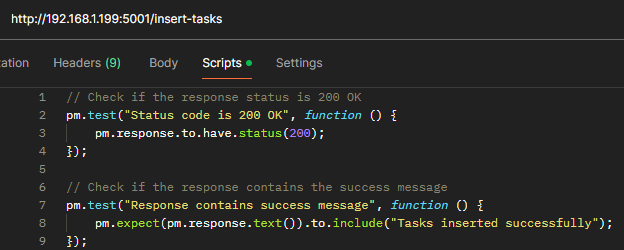
\includegraphics[width=0.8\textwidth, height=5cm]{chap4.images/source test.png}
  \caption{ Code souce du test unitaire du cas d’utilisation « Créer taches » }

\end{figure}

\bigskip

\begin{figure}[h!]
  \centering
  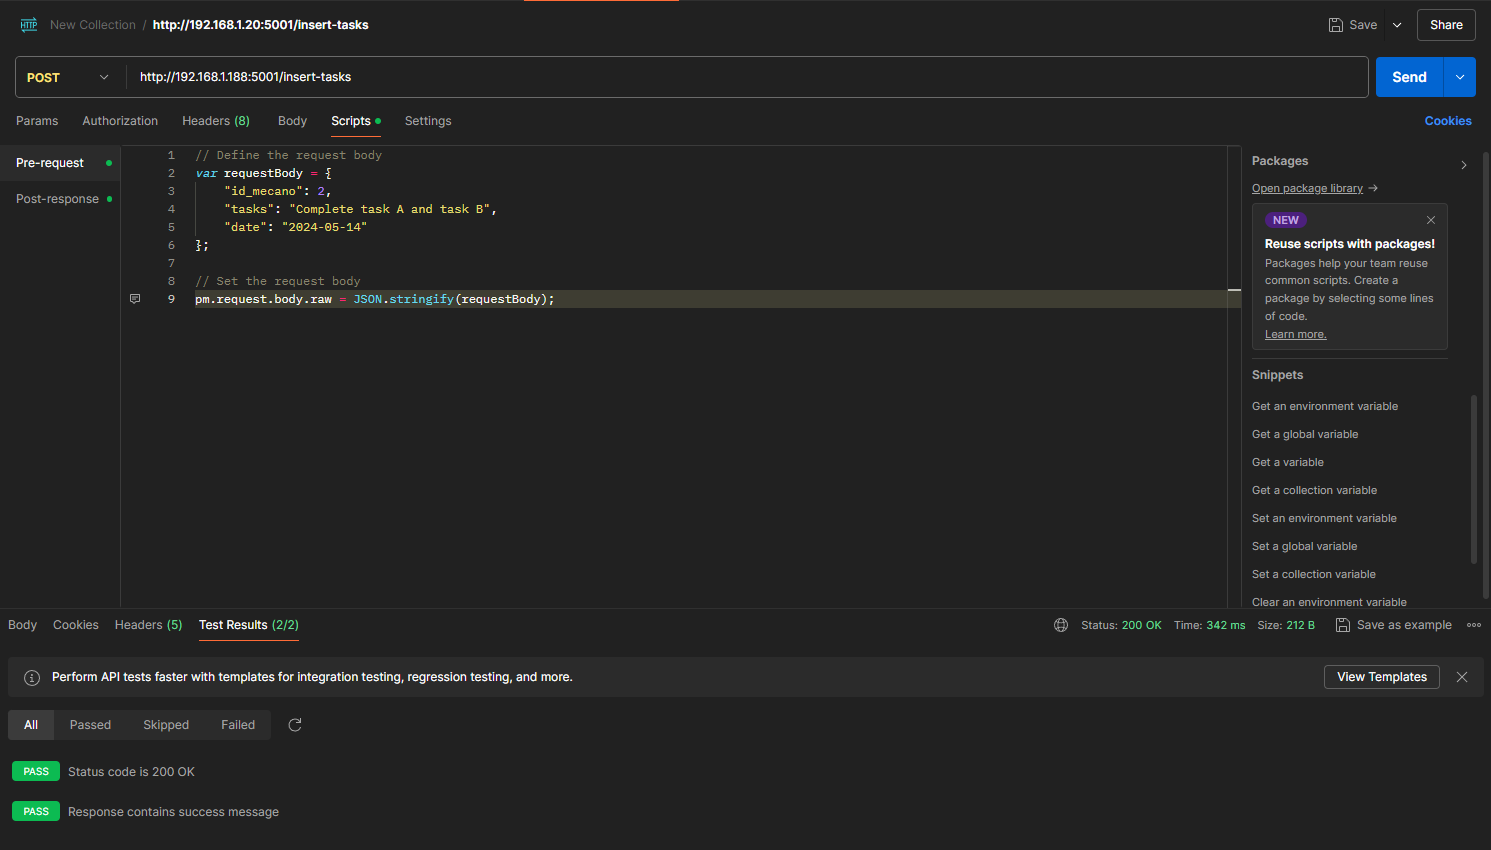
\includegraphics[width=0.8\textwidth, height=7cm]{chap4.images/reussite.png}
  \caption{ Resultat du test de réussite}

\end{figure}
\newpage
\begin{figure}[h!]
  \centering
  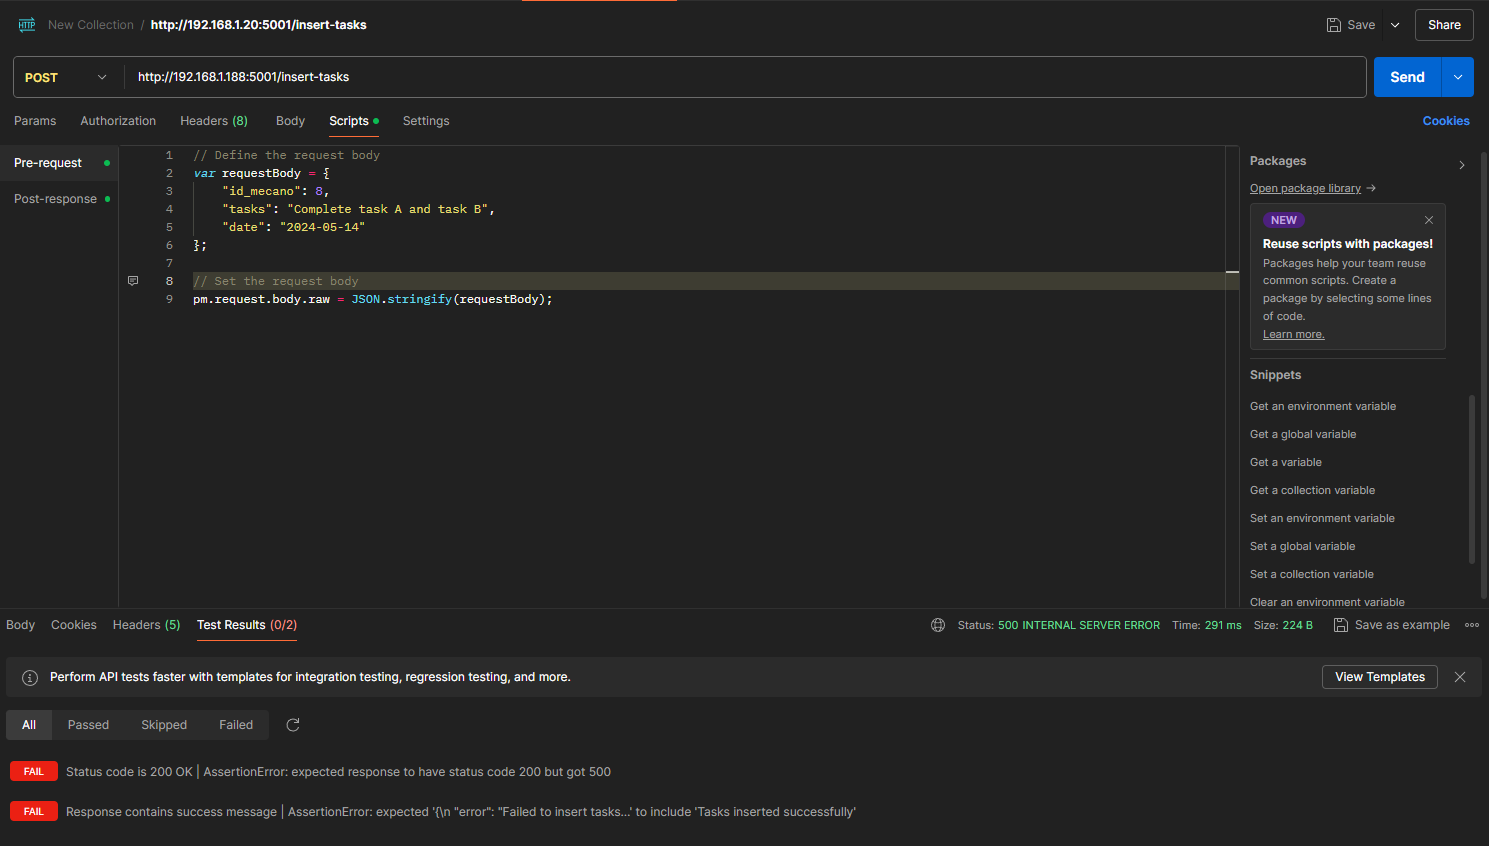
\includegraphics[width=0.8\textwidth, height=7cm]{chap4.images/echec.png}
  \caption{ Resultat du test d'échec }

\end{figure}


%_______________________________________________________________________________________________

\section*{Conclusion}
\addcontentsline{toc}{section}{Conclusion}
\bigskip
\begin{sloppypar}
  Dans le sprint 2, nous avons implémenté avec succès la création des tâches par le chef d'équipe et leur consultation par les chauffeurs et les mécaniciens. Les diagrammes de cas d'utilisation et les séquences système ont été efficacement déployés, accompagnés de descriptions textuelles et de captures d'interfaces qui illustrent clairement les avancées réalisées. Les tests unitaires ont confirmé la fiabilité des nouvelles fonctionnalités.Dans le prochain chapitre, nous explorerons le Sprint 3 : 'Suivi et Création des Rapports'.
\end{sloppypar}

